\documentclass[preprint,12pt]{elsarticle}
\usepackage{graphicx}
\usepackage[margin=1.0in]{geometry}
\usepackage{color, colortbl}
\usepackage{hyperref}
\usepackage{float}
% \usepackage[affil-it]{authblk}
\usepackage{subcaption}
\newcommand{\note}[1]{\textcolor{blue}{#1}}
\definecolor{LightCyan}{rgb}{0.88,1,1}
\definecolor{LightRose}{rgb}{1,0.88,0.88}
\definecolor{LightGreen}{rgb}{0.88,1,0.88}

\title{Real-Time event reconstruction for Nuclear Physics Experiments using Artificial Intelligence}
\author[1]{Gagik Gavalian}

\address[1]{Jefferson Lab, Newport News, VA, USA}
%\address[2]{CRTC, Department of Computer Science, Old Dominion University, Norfolk, VA, USA}
%Authored by Jefferson Science Associates, LLC under U.S. DOE Contract No. DE-AC05-06OR23177. The U.S. Government retains a non-exclusive, paid-up, irrevocable, world-wide license to publish or reproduce this manuscript for U.S. Government purposes.

%\fntext[fn1]{Authors contributed equally.}
%\fntext[fn2]{Correspoding author, \textit{gavalian@jlab.org}}


\begin{document}

%\begin{titlepage}

\begin{abstract}
\indent
Charged track reconstruction is a critical task in nuclear physics experiments, enabling the identification and analysis of particles produced in high-energy collisions. Machine learning (ML) has emerged as a powerful tool for this purpose, addressing the challenges posed by complex detector geometries, high event multiplicities, and noisy data. Traditional methods rely on pattern recognition algorithms like the Kalman filter, but ML techniques, such as neural networks, graph neural networks (GNNs), and recurrent neural networks (RNNs), offer improved accuracy and scalability. By learning from simulated and real detector data, ML models can identify and classify tracks, predict trajectories, and handle ambiguities caused by overlapping or missing hits. Moreover, ML-based approaches can process data in near-real-time, enhancing the efficiency of experiments at large-scale facilities like the Large Hadron Collider (LHC) and Jefferson Lab (JLAB). As detector technologies and computational resources evolve, ML-driven charged track reconstruction continues to push the boundaries of precision and discovery in nuclear physics. 

In this talk, we highlight advancements in charged track identification leveraging Artificial Intelligence within the CLAS12 detector, achieving a notable enhancement in experimental statistics compared to traditional methods. Additionally, we showcase real-time event reconstruction capabilities, including the inference of charged particle properties such as momentum, direction, and species identification, at speeds matching data acquisition rates. These innovations enable the extraction of physics observables directly from the experiment in real-time.
\end{abstract}
%\end{titlepage}
\maketitle

\section{Introduction}
\indent
Nuclear physics experiments have grown increasingly complex over recent decades, featuring more sophisticated detector systems and higher luminosities. In new experiments with elevated detector occupancies, innovative approaches to data processing are essential to enhance both the accuracy and speed of data reconstruction. Advances in Artificial Intelligence (AI) offer promising alternatives to traditional algorithms, with Machine Learning (ML) techniques being utilized at various stages of experimental data processing, including detector reconstruction, particle identification, detector simulations, and physics analysis.

This paper explores the integration of machine learning models into the CLAS12 charged-particle track reconstruction software. It provides a comprehensive analysis of the reconstruction performance, highlighting improvements in track reconstruction efficiency and processing speed compared to conventional methods.


\section{CLAS12 Detector}

The CLAS12 (CEBAF Large Acceptance Spectrometer for 12 GeV) detector is a state-of-the-art experimental apparatus used in nuclear physics research. It is located at the Thomas Jefferson National Accelerator Facility (Jefferson Lab) in Newport News, Virginia. The detector is part of an upgrade to the Continuous Electron Beam Accelerator Facility (CEBAF), which increased the maximum energy of the electron beam from 6 GeV to 12 GeV. This upgrade allows for a more in-depth exploration of the structure and properties of nucleons (protons and neutrons) and the nature of the strong force that binds them together in the atomic nucleus.

\begin{figure}[h!]
\centering
\centerline{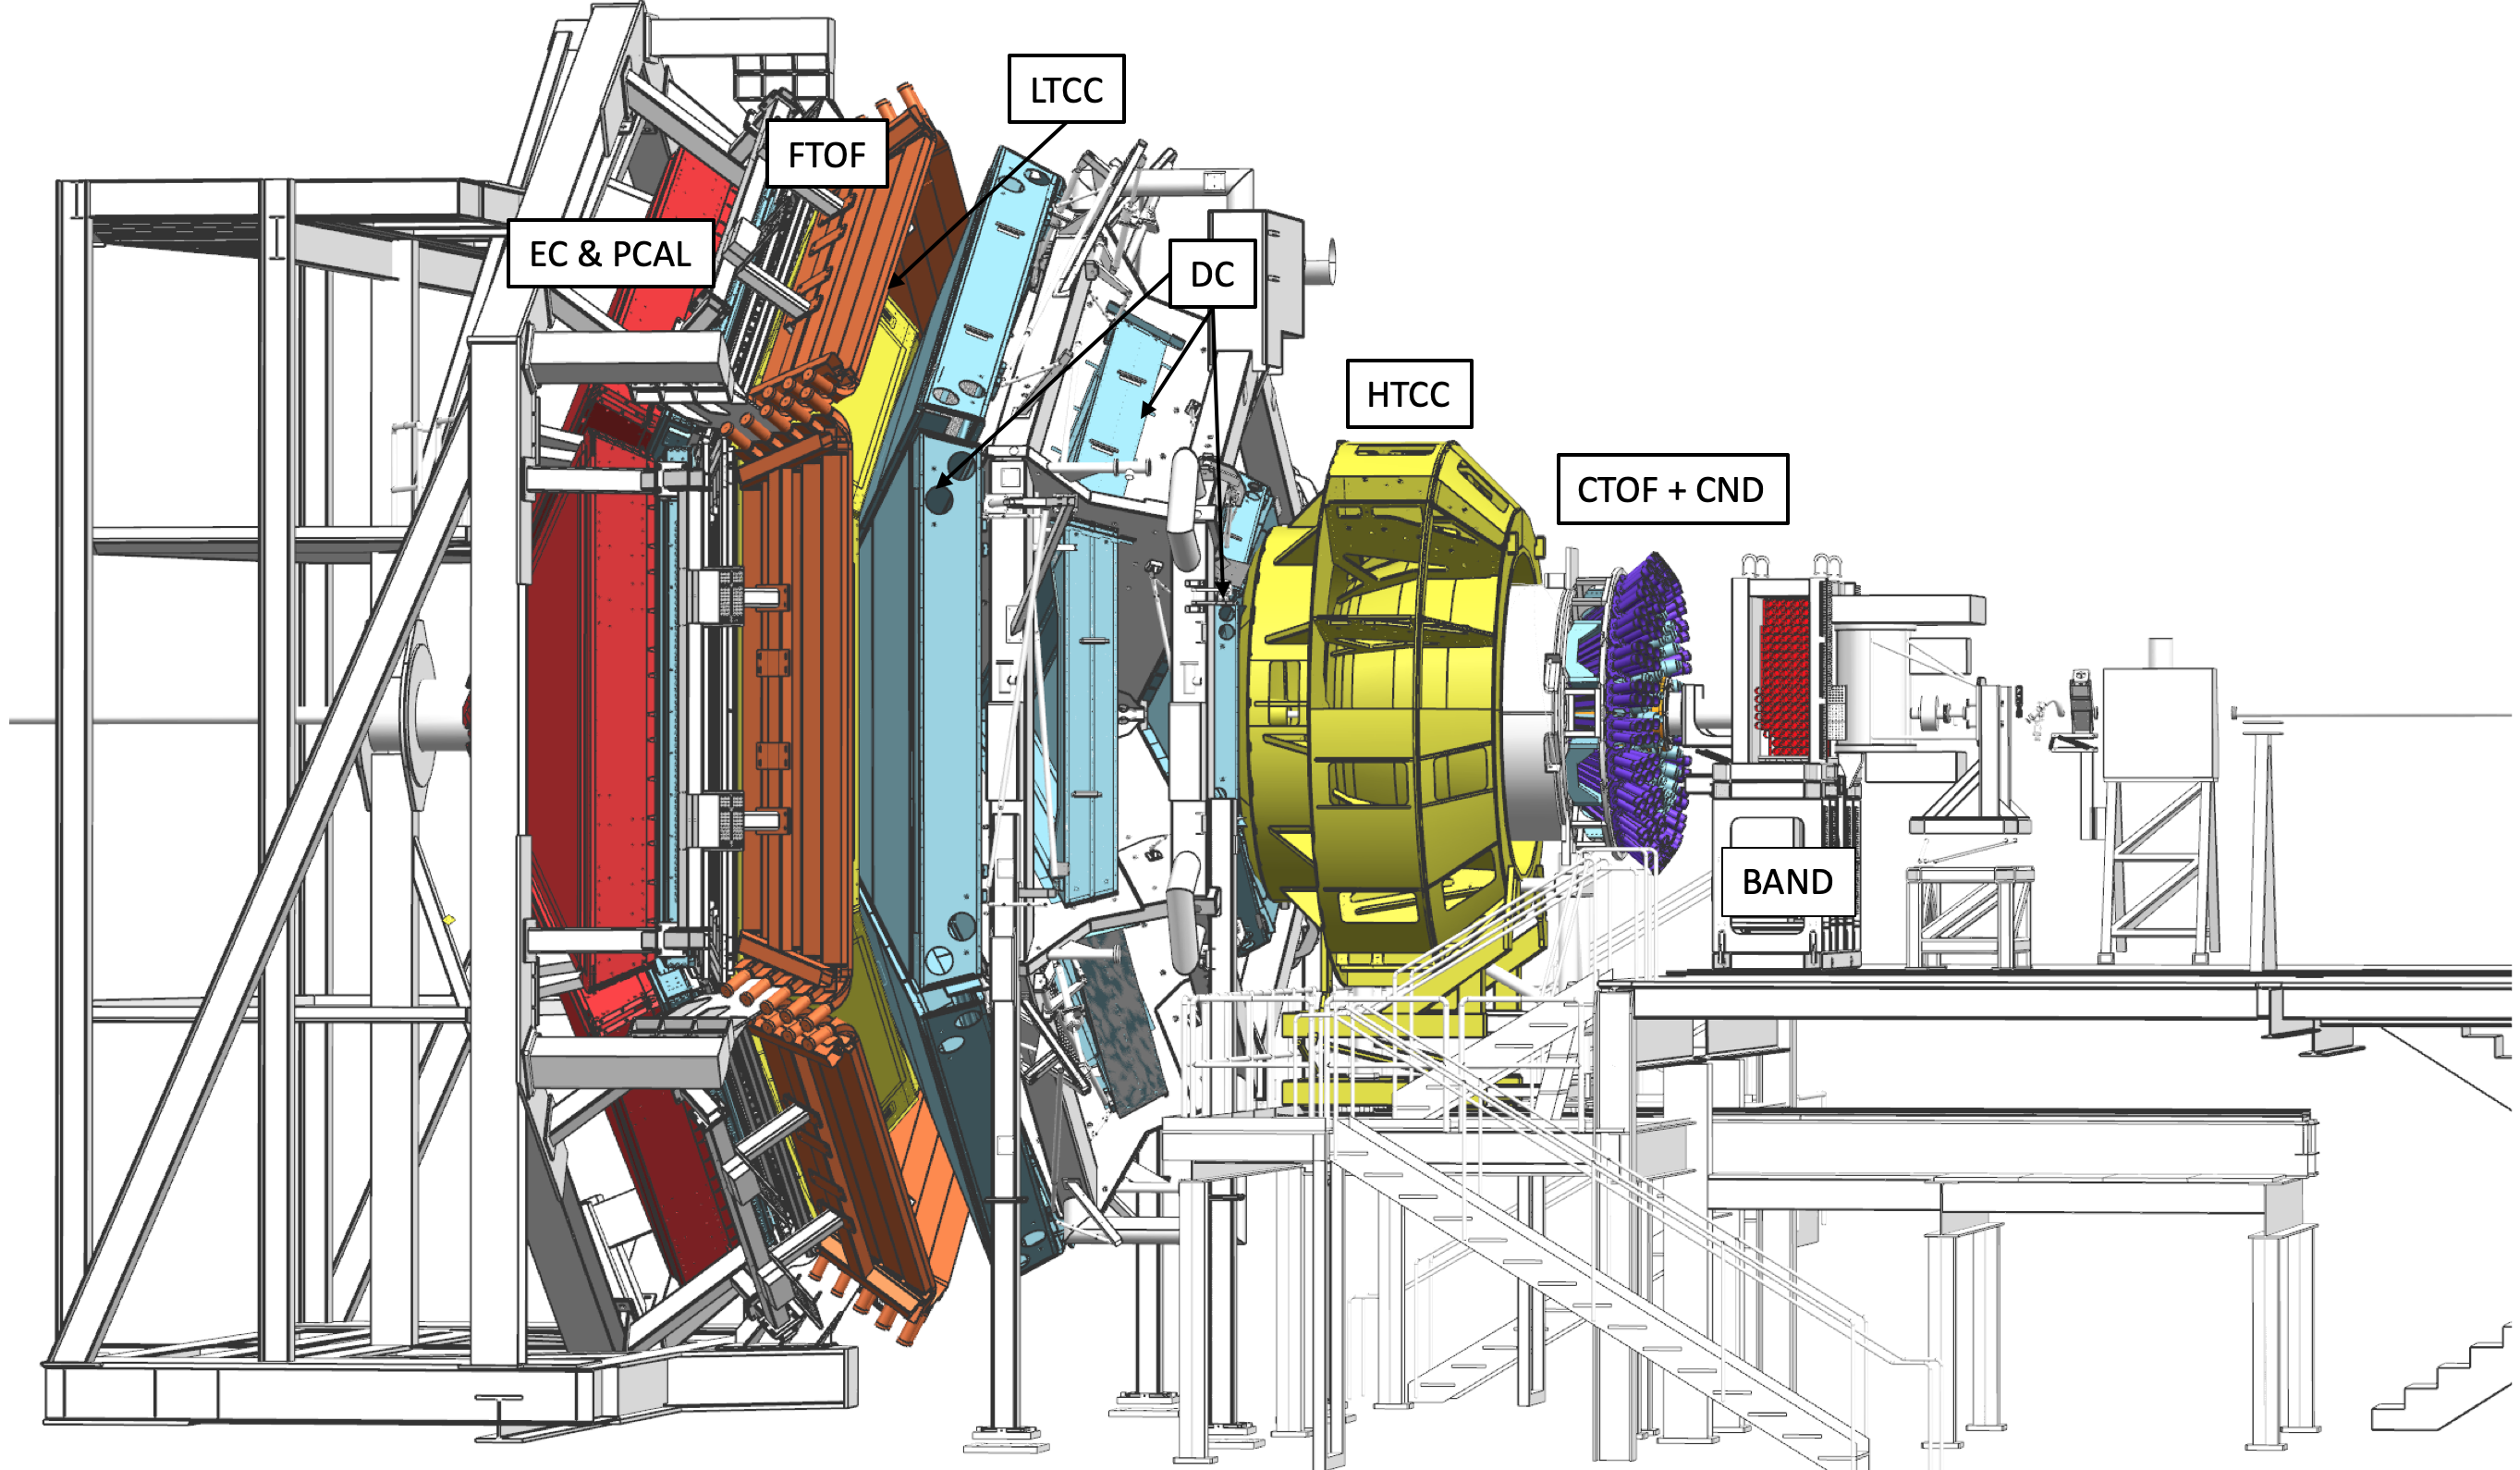
\includegraphics[width=0.7\columnwidth]{images/CLAS12-side.png}}
\caption{The CLAS12 detector in the Hall~B beamline. The electron beam enters from the right and impinges on
  the production target located in the center of the solenoid magnet shown at the right (upstream) end of CLAS12,
  where other detector components are also visible. Scattered electrons and forward-going particles are detected
  in the Forward Detector (FD), consisting of the High Threshold Cherenkov Counter (HTCC) (yellow), 
  followed by the torus magnet (gray), the drift chamber tracking system (light blue),
  and time-of-flight scintillation counters (brown), and electromagnetic calorimeters (red). } 
\label{fig:CLAS12}
\end{figure}

Key features and capabilities of the CLAS12 detector include:

\begin{itemize}

\item{\bf Large Acceptance: } As its name suggests, CLAS12 has a large angular and momentum acceptance. This feature is crucial for detecting particles over a wide range of angles and energies, allowing comprehensive analysis of nuclear reactions.
\item{\bf Electron Beam Experiments:} CLAS12 is designed to investigate the interactions of high-energy electrons with nucleons and nuclei. By scattering electrons off target materials, scientists can probe the internal structure of nucleons and the dynamics of the strong force.
\item{\bf High Luminosity:} The detector operates at high luminosities, enabling it to collect a vast amount of data from electron scattering experiments. This high data rate is essential for studying rare processes and achieving statistically significant results.
\item{\bf Sophisticated Detection Systems:} CLAS12 consists of various subsystems designed to detect different types of particles and measure their properties. These include drift chambers for tracking charged particles, time-of-flight counters for particle identification, calorimeters for measuring energy, and Cherenkov detectors for identifying electrons.
\item{\bf Versatility:} The detector is versatile and can be used for a wide range of experiments, from studying the quark-gluon structure of nucleons to investigating the properties of nuclei under extreme conditions.
\item{\bf Data Analysis and Simulation:} Advanced software and computational tools are used to analyze the data collected by CLAS12. These tools include simulation packages that model the detector's response and data analysis frameworks for extracting physical quantities from the experimental data.
\end{itemize}
In summary, CLAS12 is a critical tool in modern nuclear physics, enabling researchers to delve deeper into the quantum world of nucleons and nuclei. Its advanced technology and capabilities contribute significantly to our understanding of fundamental physics, particularly in the realm of quantum chromodynamics (QCD), the theory describing the strong interaction.


\section{Drift Chamber Particle Tracking}

The CLAS12~\cite{Burkert:2020akg} forward detector is built around a six-coil toroidal magnet 
which divides the active detection area into six azimuthal regions, called ``sectors''. Each sector is 
equipped with three regions of drift chambers~\cite{Mestayer:2020saf} designed to detect charged 
particles produced by the interaction of an electron beam with a target. Each region consists of two 
chambers (called super-layers), each of them having six layers of wires. Each layer  in a super-layer 
contains 112 signal wires, making a super-layer a $6\times112$ cell matrix. 
The schematic view of all sectors and super-layers is shown in Figure~\ref{fig:drift_chambers}.

\begin{figure}[h!]
\centering
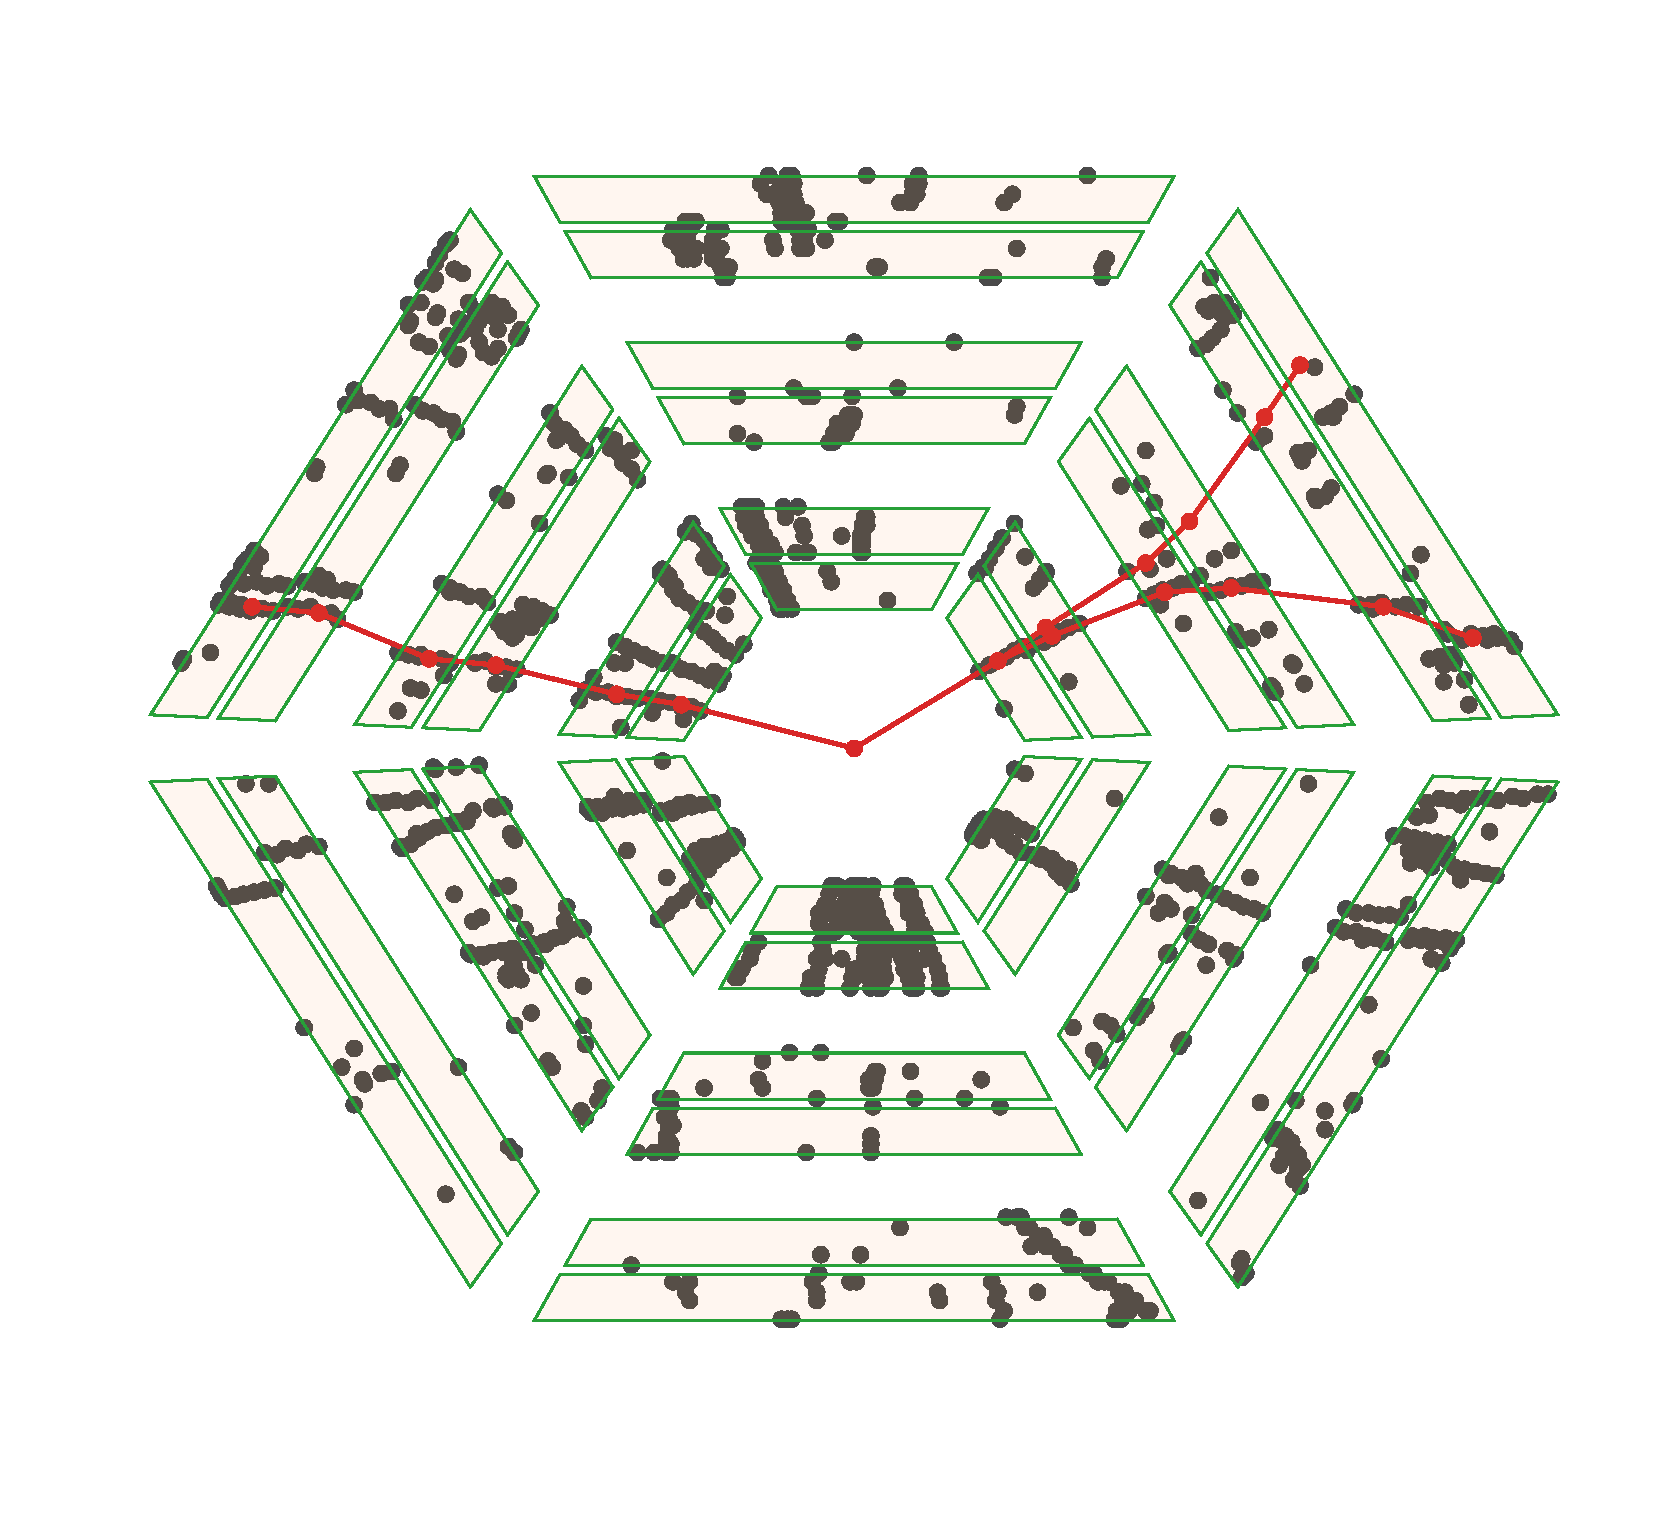
\includegraphics[width=0.32\columnwidth]{images/evt_05.pdf}
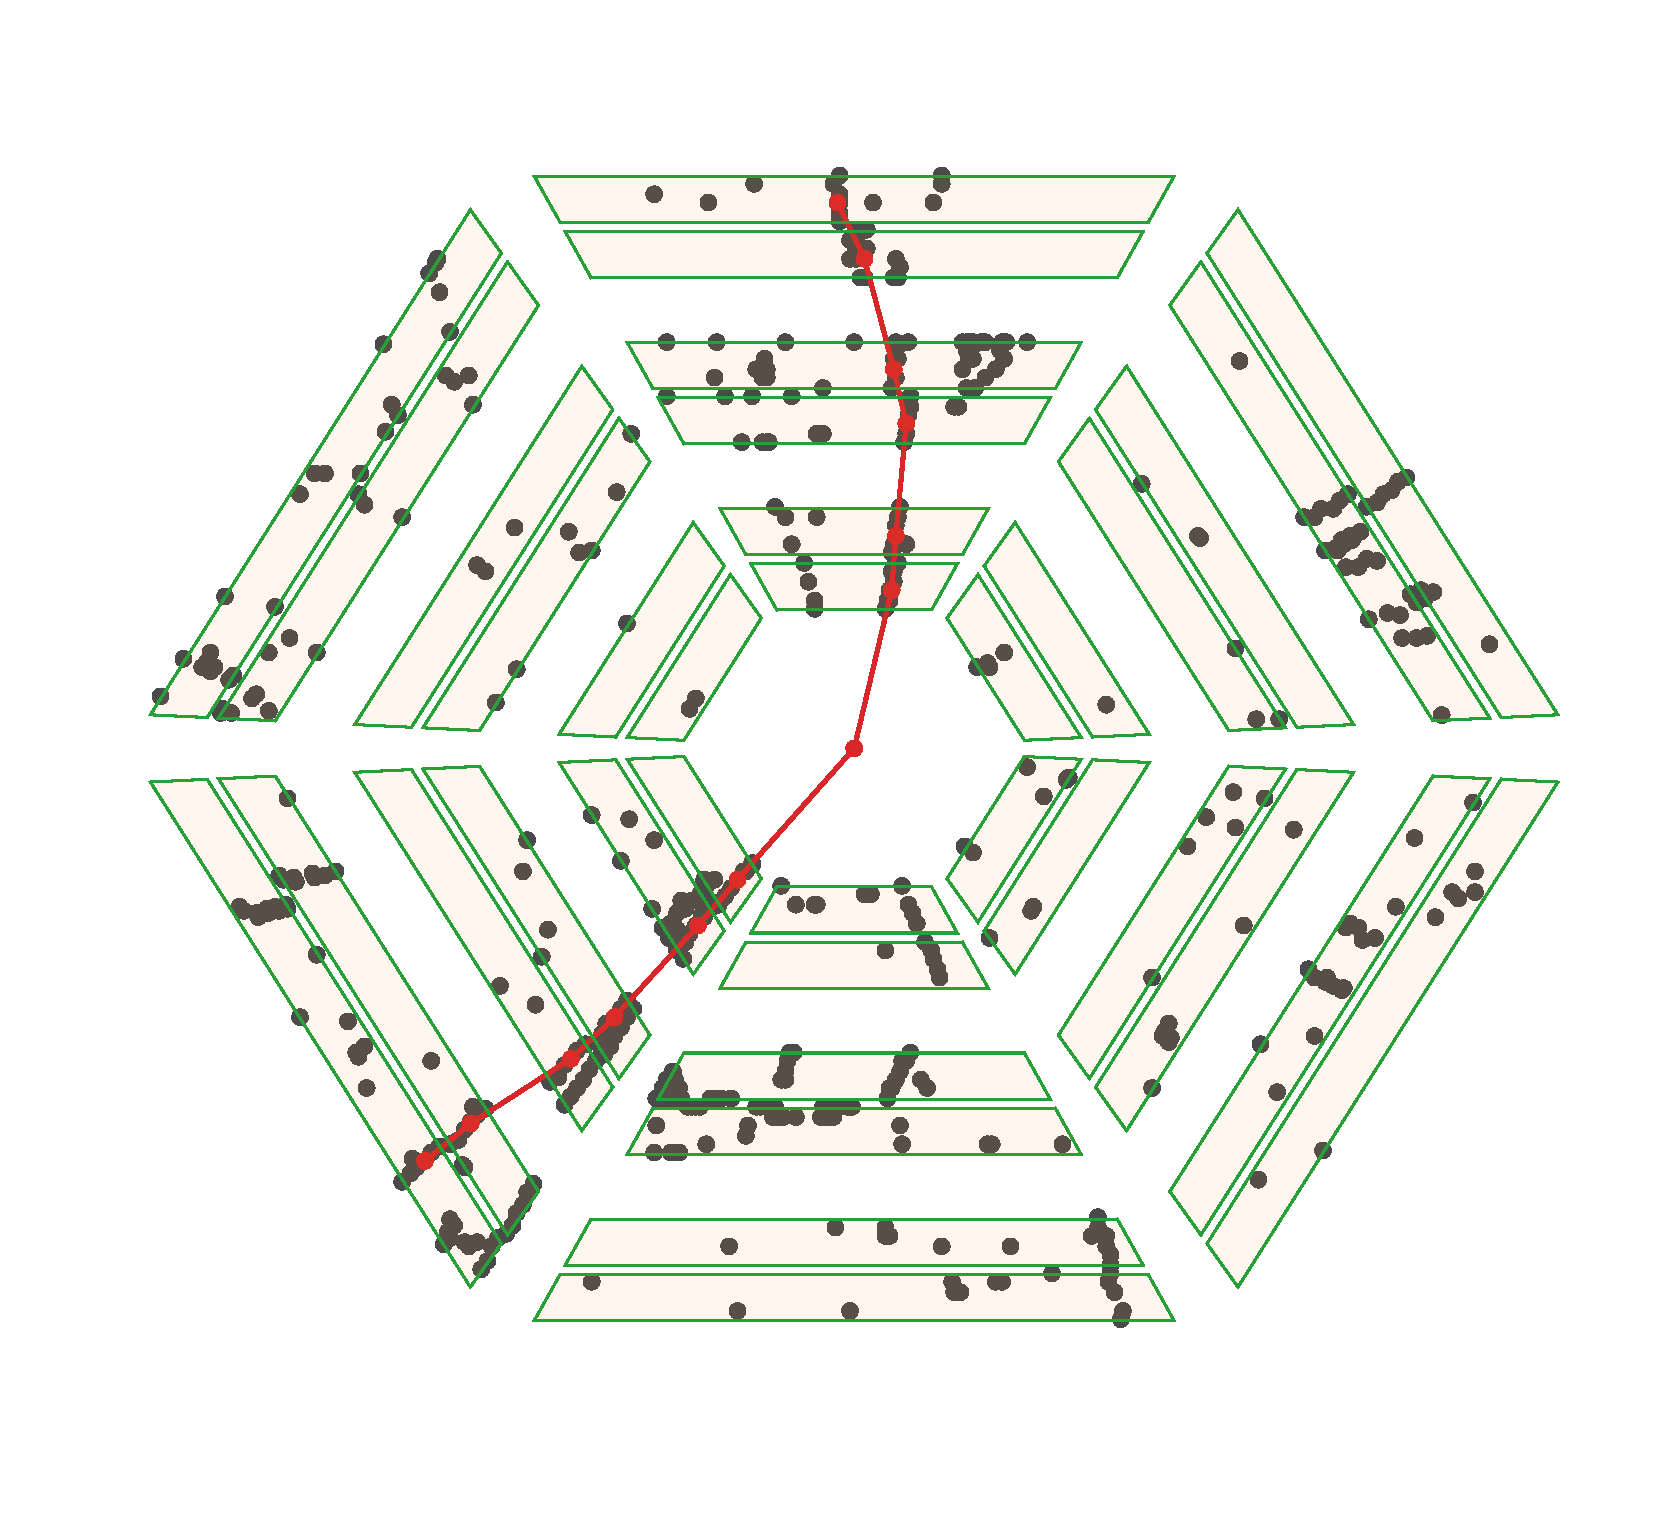
\includegraphics[width=0.32\columnwidth]{images/evt_26.pdf}
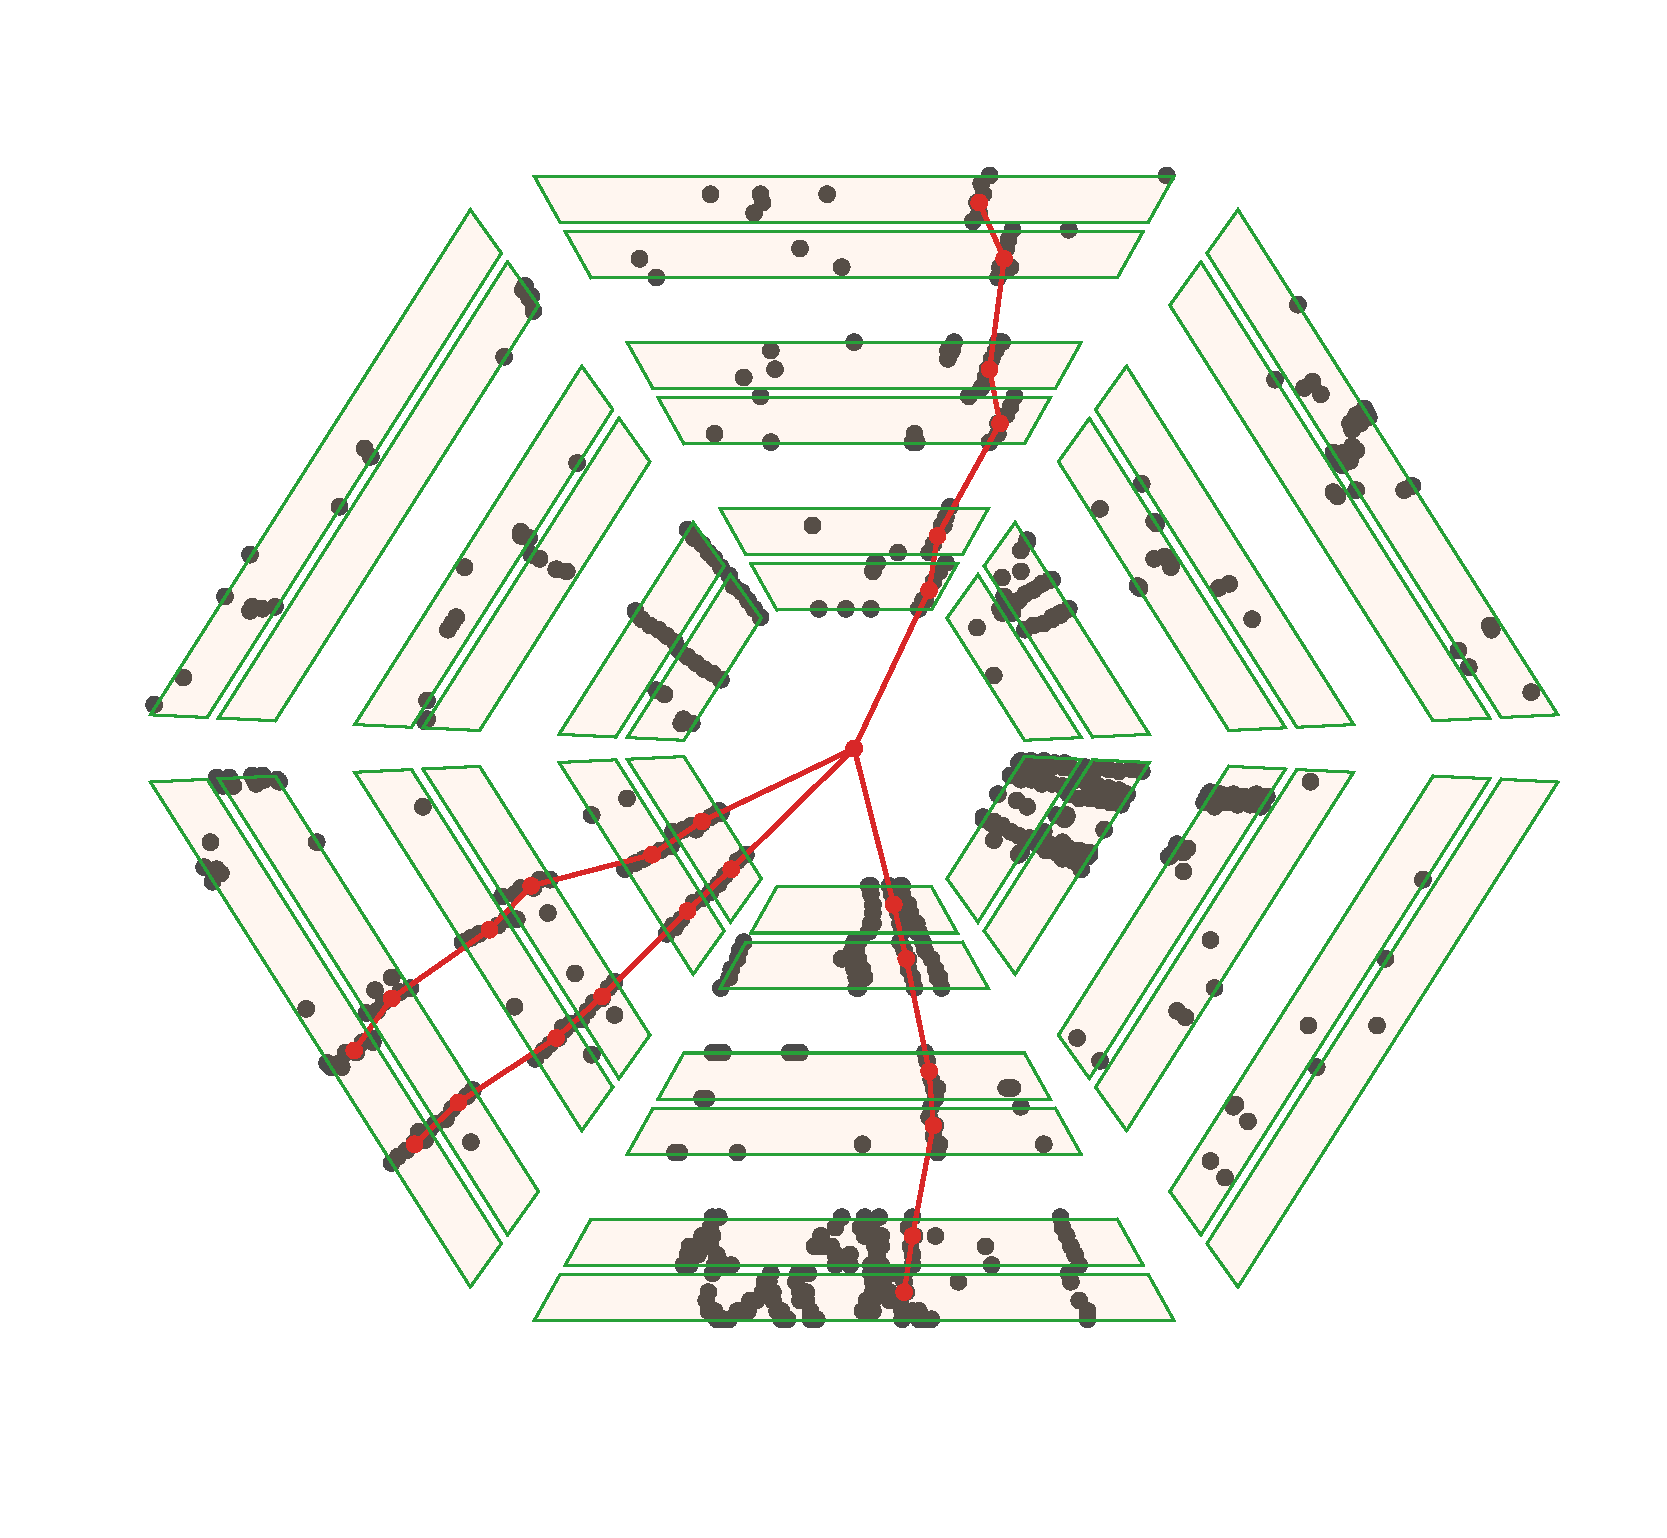
\includegraphics[width=0.32\columnwidth]{images/evt_35.pdf}
\caption{Example views of the six sectors of the Drift Chambers of CLAS12. The points show wire hits for each of the layers in the drift chambers and the lines indicate reconstructed tracks by the conventional CLAS12 tracking algorithm. } 
\label{fig:drift_chambers}
\end{figure}

Particles that originate from the interaction vertex travel through the magnetic field and pass through all 
three regions of the drift chambers in a given sector and are reconstructed by tracking algorithms. First, 
in each super-layer adjacent wires with a signal are grouped into segments. Track candidates are constructed 
by connecting segments in each super-layer to form a track trajectory. Then each track candidate is fitted through 
a magnetic field to calculate the quality of the track ($\chi^2$), and the track candidates with $\chi^2$ below the cut value
are saved for further refinement using Kalman-filter~\cite{Kalman1960}.

The positions of these segments in each super-layer are used to fit the track trajectory 
to derive initial parameters, such as momentum and direction (called "hit-based" tracking).  After the initial selection, good track candidates 
(shown in Figure~\ref{fig:drift_chambers} with lines) are passed through a Kalman-filter to 
refine measured parameters further (called "time-based" tracking).

At the first stage of the tracking, the tracks are identified using only the hit positions (wire number). The precision 
of the reconstructed track parameters using only hit positions are worse ($\sim3\%$) than the final calculated parameters from time-based tracking, but they are sufficient to calculate physics quantities from the event and identify desired reactions in the event. 

The CLAS12 track reconstruction process is already making use of AI at different stages.
First, a Convolutional
Autoencoder is used to de-noise the drift chamber hits~\cite{Thomadakis:2022zcd}, which leads to improved cluster
identification in each super-layer. Then after the clustering, the track candidates are identified using a Multilayer perceptron (MLP) classifier,
which identifies 6-super-layer and 5-super-layer track candidates~\cite{Gavalian:2020oxg}. The combined result of
de-noising and AI-assisted track candidate identification used in CLAS12 leads to an increase in statistics of multi-particle 
final states of $50\%-75\%$ depending on kinematics~\cite{Gavalian:2020xmc}. 
Furthermore, an Artificial Intelligence approach to track reconstruction was developed to estimate track parameters 
(such as momentum and direction) based on cluster positions of the track~\cite{Thomadakis:2023ebe}, it was shown that 
the AI-estimated track parameters are closer to the values reconstructed using the Kalman-filter than the 
conventional hit-based tracking.

The developed AI tools for CLAS12 reconstruction can identify tracks from their cluster pattern and estimate the track parameters.
If combined with the clustering algorithm, this chain may provide a complete track reconstruction solely based on AI algorithms and
may potentially be used in real-time with data acquisition. 

%\input{introduction}
%\input{calorimeter}

\section{Charged Track Reconstruction using Artificial Intelligence}

\subsection{De-noising}

\begin{figure}[h!]
\centering
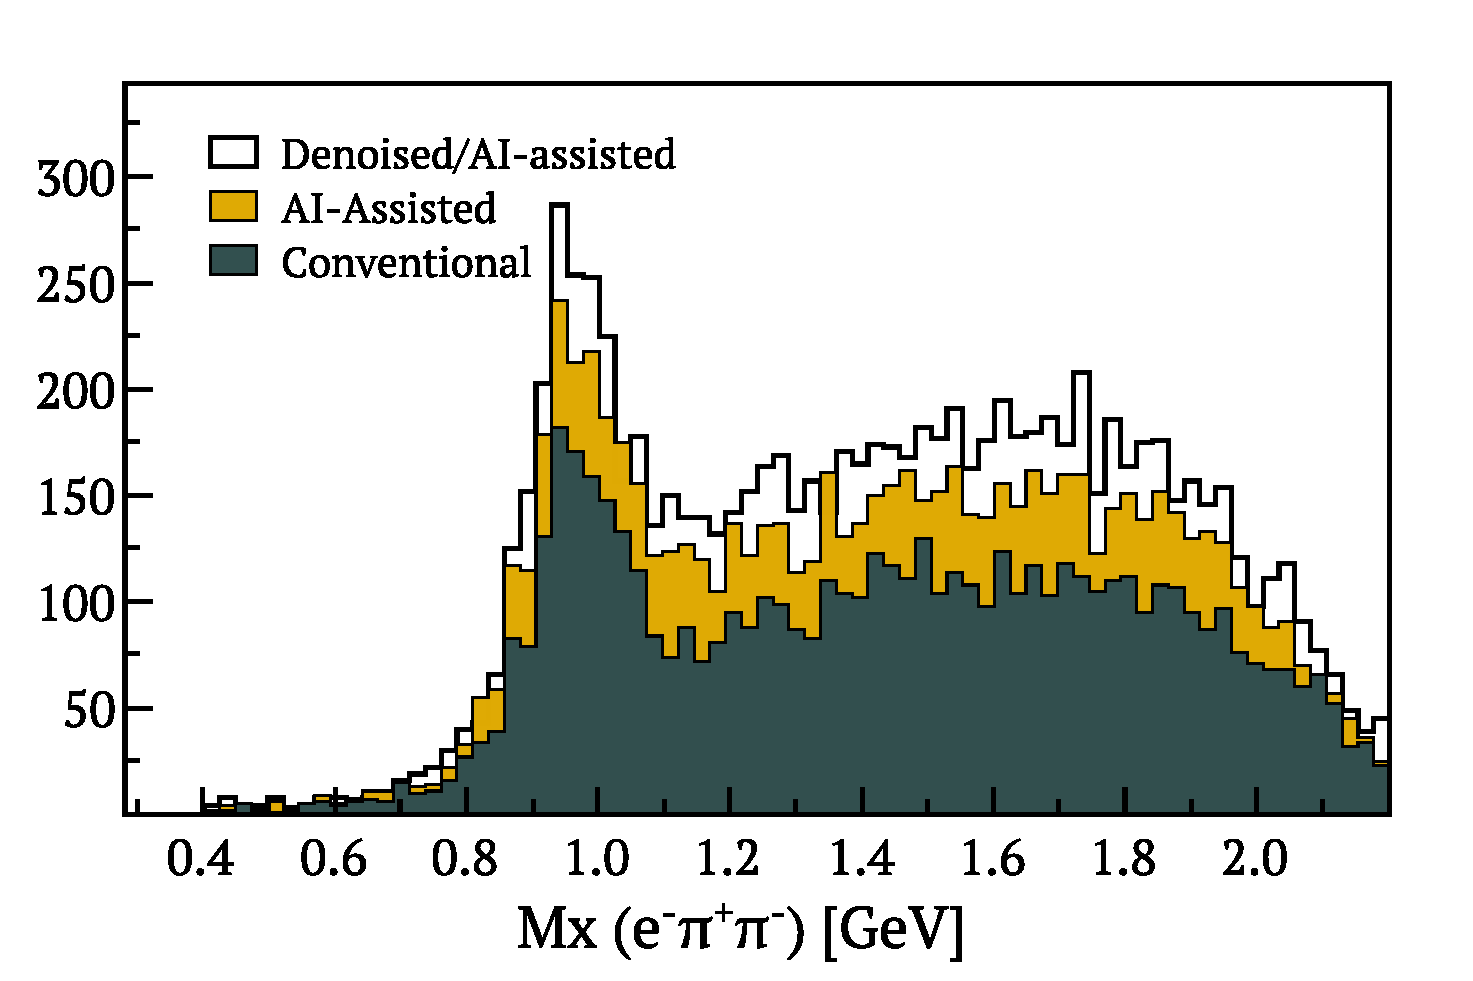
\includegraphics[width=0.44\columnwidth]{images/figure_denoise_mxp.pdf}
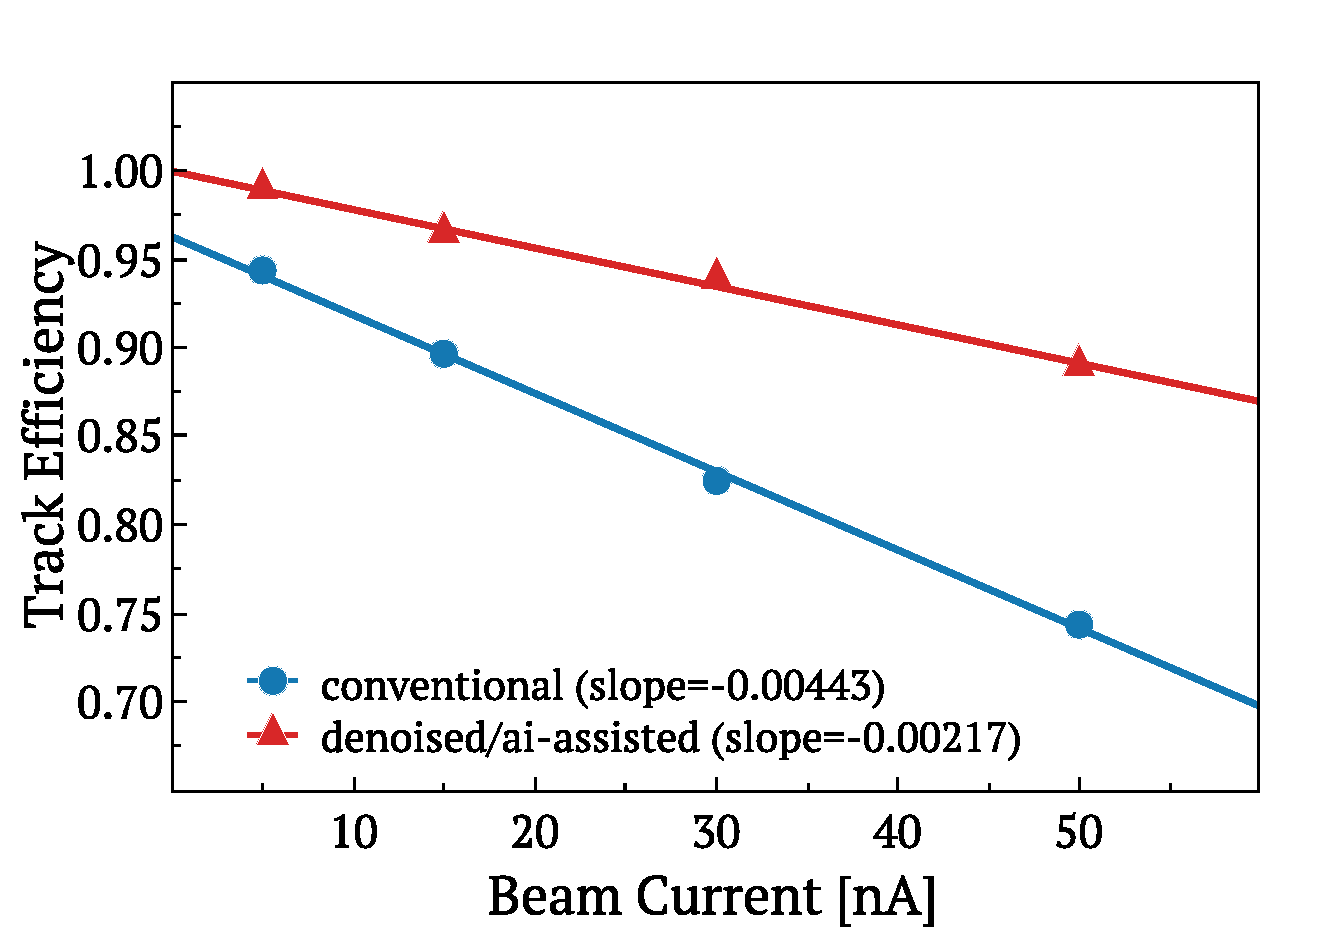
\includegraphics[width=0.42\columnwidth]{images/luminosity_scan.pdf}
\caption{Drift Chamber De-noising and Track identification impact on physics observables measured by CLAS12} 
\label{fig:drift_chambers_denoise}
\end{figure}

\subsection{Real-Time Event Reconstruction}

\begin{figure}[h!]
\centering
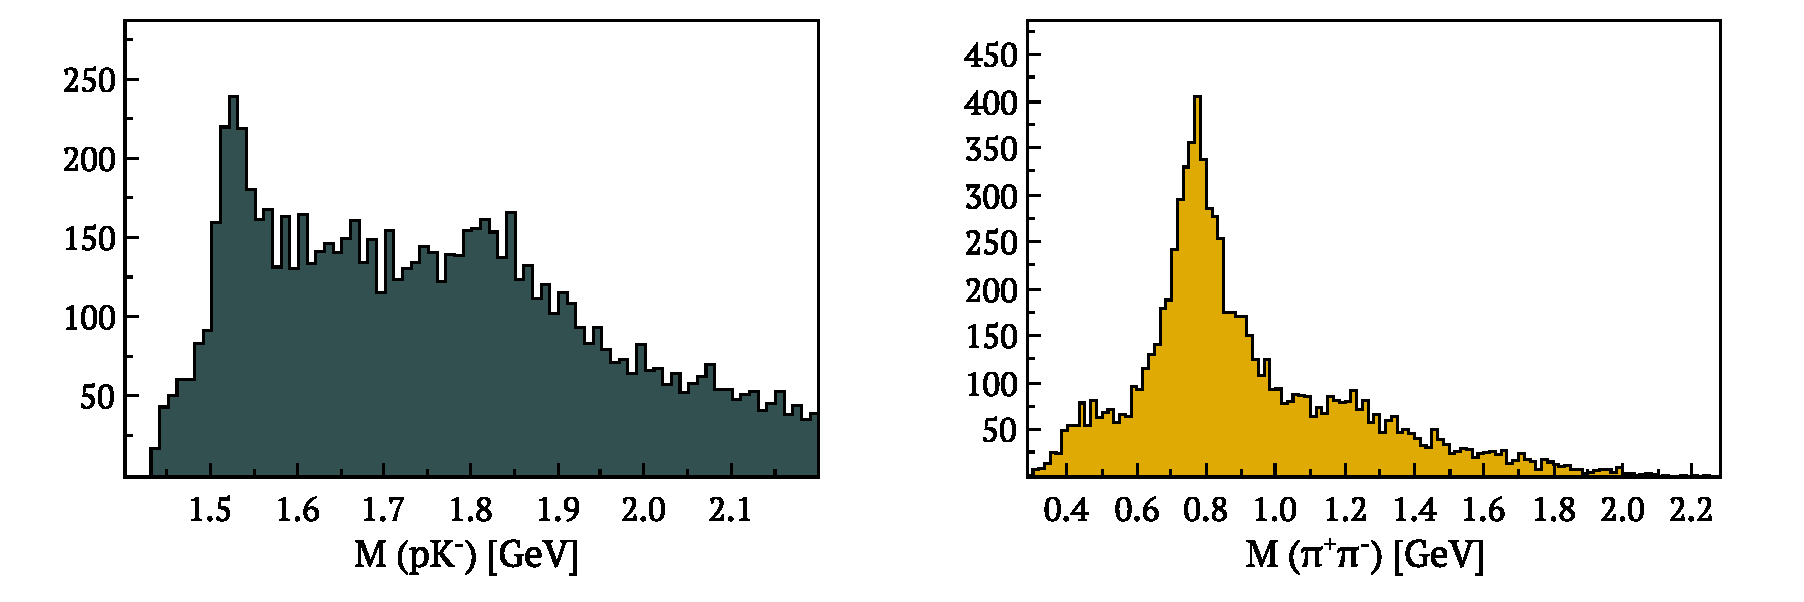
\includegraphics[width=0.88\columnwidth]{images/figure_lambda_instarec.pdf}

\caption{Drift Chamber De-noising and Track identification impact on physics observables measured by CLAS12} 
\label{fig:drift_chambers_instarec}
\end{figure}

\section{Acknowledgments}
This material is based upon work supported by the U.S. Department of Energy, Office of Science, Office of Nuclear Physics under contract DE-AC05-06OR23177, and NSF grant no. CCF-1439079 and the Richard T. Cheng Endowment. 
 
%\newpage
%\bibliography{references}
%\bibliographystyle{ieeetr}

\end{document}
